\documentclass[tikz]{standalone}
\begin{document}
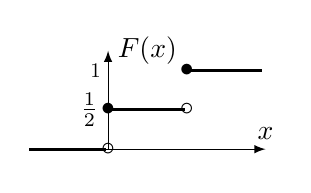
\begin{tikzpicture}
  \draw[-latex] (-1,0)--(2,0) node[above] {\(x\)};
  \draw[-latex] (0,0)--(0,1.25) node[right] {\(F(x)\)};
  \node at (0,0) {\(\circ\)};
  \node at (0,0.5) {\(\bullet\)};
  \node at (1,0.5) {\(\circ\)};
  \node at (1,1) {\(\bullet\)};
  \draw[very thick] (-1,0)--(-0.025,0);
  \draw[very thick] (0,0.5)--(0.975,0.5);
  \draw[very thick] (1,1)--(1.95,1);
  \node[left, scale=0.75] at (0,1) {\(1\)};
  \node[left] at (0,0.5) {\(\frac{1}{2}\)};
\end{tikzpicture}
\end{document}
